% Options for packages loaded elsewhere
% Options for packages loaded elsewhere
\PassOptionsToPackage{unicode}{hyperref}
\PassOptionsToPackage{hyphens}{url}
\PassOptionsToPackage{dvipsnames,svgnames,x11names}{xcolor}
%
\documentclass[
]{article}
\usepackage{xcolor}
\usepackage{amsmath,amssymb}
\setcounter{secnumdepth}{-\maxdimen} % remove section numbering
\usepackage{iftex}
\ifPDFTeX
  \usepackage[T1]{fontenc}
  \usepackage[utf8]{inputenc}
  \usepackage{textcomp} % provide euro and other symbols
\else % if luatex or xetex
  \usepackage{unicode-math} % this also loads fontspec
  \defaultfontfeatures{Scale=MatchLowercase}
  \defaultfontfeatures[\rmfamily]{Ligatures=TeX,Scale=1}
\fi
\usepackage{lmodern}
\ifPDFTeX\else
  % xetex/luatex font selection
\fi
% Use upquote if available, for straight quotes in verbatim environments
\IfFileExists{upquote.sty}{\usepackage{upquote}}{}
\IfFileExists{microtype.sty}{% use microtype if available
  \usepackage[]{microtype}
  \UseMicrotypeSet[protrusion]{basicmath} % disable protrusion for tt fonts
}{}
\makeatletter
\@ifundefined{KOMAClassName}{% if non-KOMA class
  \IfFileExists{parskip.sty}{%
    \usepackage{parskip}
  }{% else
    \setlength{\parindent}{0pt}
    \setlength{\parskip}{6pt plus 2pt minus 1pt}}
}{% if KOMA class
  \KOMAoptions{parskip=half}}
\makeatother
% Make \paragraph and \subparagraph free-standing
\makeatletter
\ifx\paragraph\undefined\else
  \let\oldparagraph\paragraph
  \renewcommand{\paragraph}{
    \@ifstar
      \xxxParagraphStar
      \xxxParagraphNoStar
  }
  \newcommand{\xxxParagraphStar}[1]{\oldparagraph*{#1}\mbox{}}
  \newcommand{\xxxParagraphNoStar}[1]{\oldparagraph{#1}\mbox{}}
\fi
\ifx\subparagraph\undefined\else
  \let\oldsubparagraph\subparagraph
  \renewcommand{\subparagraph}{
    \@ifstar
      \xxxSubParagraphStar
      \xxxSubParagraphNoStar
  }
  \newcommand{\xxxSubParagraphStar}[1]{\oldsubparagraph*{#1}\mbox{}}
  \newcommand{\xxxSubParagraphNoStar}[1]{\oldsubparagraph{#1}\mbox{}}
\fi
\makeatother


\usepackage{longtable,booktabs,array}
\newcounter{none} % for unnumbered tables
\usepackage{calc} % for calculating minipage widths
% Correct order of tables after \paragraph or \subparagraph
\usepackage{etoolbox}
\makeatletter
\patchcmd\longtable{\par}{\if@noskipsec\mbox{}\fi\par}{}{}
\makeatother
% Allow footnotes in longtable head/foot
\IfFileExists{footnotehyper.sty}{\usepackage{footnotehyper}}{\usepackage{footnote}}
\makesavenoteenv{longtable}
\usepackage{graphicx}
\makeatletter
\newsavebox\pandoc@box
\newcommand*\pandocbounded[1]{% scales image to fit in text height/width
  \sbox\pandoc@box{#1}%
  \Gscale@div\@tempa{\textheight}{\dimexpr\ht\pandoc@box+\dp\pandoc@box\relax}%
  \Gscale@div\@tempb{\linewidth}{\wd\pandoc@box}%
  \ifdim\@tempb\p@<\@tempa\p@\let\@tempa\@tempb\fi% select the smaller of both
  \ifdim\@tempa\p@<\p@\scalebox{\@tempa}{\usebox\pandoc@box}%
  \else\usebox{\pandoc@box}%
  \fi%
}
% Set default figure placement to htbp
\def\fps@figure{htbp}
\makeatother


% definitions for citeproc citations
\NewDocumentCommand\citeproctext{}{}
\NewDocumentCommand\citeproc{mm}{%
  \begingroup\def\citeproctext{#2}\cite{#1}\endgroup}
\makeatletter
 % allow citations to break across lines
 \let\@cite@ofmt\@firstofone
 % avoid brackets around text for \cite:
 \def\@biblabel#1{}
 \def\@cite#1#2{{#1\if@tempswa , #2\fi}}
\makeatother
\newlength{\cslhangindent}
\setlength{\cslhangindent}{1.5em}
\newlength{\csllabelwidth}
\setlength{\csllabelwidth}{3em}
\newenvironment{CSLReferences}[2] % #1 hanging-indent, #2 entry-spacing
 {\begin{list}{}{%
  \setlength{\itemindent}{0pt}
  \setlength{\leftmargin}{0pt}
  \setlength{\parsep}{0pt}
  % turn on hanging indent if param 1 is 1
  \ifodd #1
   \setlength{\leftmargin}{\cslhangindent}
   \setlength{\itemindent}{-1\cslhangindent}
  \fi
  % set entry spacing
  \setlength{\itemsep}{#2\baselineskip}}}
 {\end{list}}
\usepackage{calc}
\newcommand{\CSLBlock}[1]{\hfill\break\parbox[t]{\linewidth}{\strut\ignorespaces#1\strut}}
\newcommand{\CSLLeftMargin}[1]{\parbox[t]{\csllabelwidth}{\strut#1\strut}}
\newcommand{\CSLRightInline}[1]{\parbox[t]{\linewidth - \csllabelwidth}{\strut#1\strut}}
\newcommand{\CSLIndent}[1]{\hspace{\cslhangindent}#1}



\setlength{\emergencystretch}{3em} % prevent overfull lines

\providecommand{\tightlist}{%
  \setlength{\itemsep}{0pt}\setlength{\parskip}{0pt}}



 


\usepackage[left=3cm,right=5cm,top=2cm,bottom=2cm]{geometry}
\usepackage{lineno}
\usepackage{setspace}
\usepackage{orcidlink}
\usepackage{etoolbox}
\makeatletter
\@ifpackageloaded{caption}{}{\usepackage{caption}}
\AtBeginDocument{%
\ifdefined\contentsname
  \renewcommand*\contentsname{Table of contents}
\else
  \newcommand\contentsname{Table of contents}
\fi
\ifdefined\listfigurename
  \renewcommand*\listfigurename{List of Figures}
\else
  \newcommand\listfigurename{List of Figures}
\fi
\ifdefined\listtablename
  \renewcommand*\listtablename{List of Tables}
\else
  \newcommand\listtablename{List of Tables}
\fi
\ifdefined\figurename
  \renewcommand*\figurename{Figure}
\else
  \newcommand\figurename{Figure}
\fi
\ifdefined\tablename
  \renewcommand*\tablename{Table}
\else
  \newcommand\tablename{Table}
\fi
}
\@ifpackageloaded{float}{}{\usepackage{float}}
\floatstyle{ruled}
\@ifundefined{c@chapter}{\newfloat{codelisting}{h}{lop}}{\newfloat{codelisting}{h}{lop}[chapter]}
\floatname{codelisting}{Listing}
\newcommand*\listoflistings{\listof{codelisting}{List of Listings}}
\makeatother
\makeatletter
\makeatother
\makeatletter
\@ifpackageloaded{caption}{}{\usepackage{caption}}
\@ifpackageloaded{subcaption}{}{\usepackage{subcaption}}
\makeatother
\usepackage{bookmark}
\IfFileExists{xurl.sty}{\usepackage{xurl}}{} % add URL line breaks if available
\urlstyle{same}
% fallback for those not using the hyperref driver hyperxmp:
\makeatletter
\@ifundefined{xmpquote}{\newcommand{\xmpquote}[1]{#1}}{}
\makeatother
\hypersetup{
  pdftitle={Fake tales of bodymass models},
  pdfkeywords={\xmpquote{food webs}},
  colorlinks=true,
  linkcolor={blue},
  filecolor={Maroon},
  citecolor={Blue},
  urlcolor={Blue},
  pdfcreator={LaTeX via pandoc}}


\title{Fake tales of bodymass models}


% ==================================================================
% 1. CAPTURE DATA 
% ==================================================================
\newcommand{\myauthors}{%
%
\textbf{Tanya Strydom}%
~\orcidlink{0000-0001-6067-1349}%
\textsuperscript{1}%
\textsuperscript{*}%
%
, %
%
\textbf{Andrew P. Beckerman}%
~\orcidlink{0000-0002-4797-9143}%
\textsuperscript{1}%
%
%
%
}

\newcommand{\myaffiliations}{%
%
\textsuperscript{1} School of Biosciences, University of Sheffield,
Sheffield, UK%
%
}

\newcommand{\myemail}{%
%
%
\textsuperscript{*}Correspondence: \texttt{t.strydom@sheffield.ac.uk}%
%
%
%
%
}

% ==================================================================
% 2. DEFINE THE LAYOUT
% ==================================================================
\makeatletter
\renewcommand{\maketitle}{%
  \newpage
  \null
  \vskip 1em%
  % Use a Group with \raggedright instead of 'flushleft' environment
  % This ensures it aligns EXACTLY with the body text margins.
  {\raggedright
    \let \footnote \thanks
    \renewcommand{\thefootnote}{\fnsymbol{footnote}}
    % TITLE
    {\LARGE \bfseries \sffamily \@title \par}%
    \vskip 1em%
    % AUTHORS
    {\large
      \lineskip .5em%
      \noindent\myauthors\par}% 
    % AFFILIATIONS
    \vskip 1em%
    {\footnotesize \myaffiliations \par}%
    % EMAIL
    \vskip 0.5em%
    {\footnotesize \myemail \par}%
  }% End group
  \par
  \vskip 1em}
\makeatother

\date{}

\usepackage[nolists,noheads,markers]{endfloat}

\begin{document}
\maketitle

% REDEFINE ABSTRACT TO REMOVE INDENTATION
\renewenvironment{abstract}
 {\small\noindent\textbf{Abstract:}}
 {\par}

  \begin{abstract}
    TODO.
          \par\bigskip
      \noindent\textbf{Keywords:} food webs
      \end{abstract}

% FORCE NEW PAGE BEFORE CONTENT
\newpage

% ==========================================================
% BODY TEXT SETUP
% ==========================================================

% 1. Set default body style
\linenumbers
\doublespacing % <--- CHANGED TO DOUBLE SPACING

% 2. Fix Table of Contents (Clean Mode)
\makeatletter
\@ifpackageloaded{etoolbox}{%
  \pretocmd{\tableofcontents}{\nolinenumbers\singlespacing}{}{}%
  \apptocmd{\tableofcontents}{\linenumbers\doublespacing}{}{}% 
}{}%
\makeatother

\begin{itemize}
\tightlist
\item
  Body-size-based allometric trophic network (ATN) (Brose et al., 2006)
  models predict interactions from consumer--resource size
  relationships.
\item
  However, body size is only one determinant of trophic interactions;
  other traits and ecological constraints may be important.
\item
  \textbf{Aim:} quantify how often body-size-based ATN models predict
  interactions absent from empirical metawebs, and test whether network
  structure can nevertheless be recovered.
\item
  Prediction: ATN models will generate a high proportion of forbidden
  interactions, even when their broad structural properties resemble
  those of empirical metawebs.
\end{itemize}

\section{Simulations}\label{simulations}

\subsection{Data sources and
preparation}\label{data-sources-and-preparation}

We analysed mammal food webs for Great Britain (GB) and Canada. For GB,
we used the European metaweb from Maiorano et al. (2020), filtered to
species on the UK Mammal Society checklist. This regional filtering was
intended to avoid classifying interactions as forbidden solely to guard
against interactions being excluded from the European metaweb on the
basis of co-occurrence constraints. For Canada, we used the
probabilistic metaweb of Strydom et al. (2022). Species names were
harmonised using genus and species names, and both metawebs were
restricted to species with positive adult body-mass estimates in
PanTHERIA (Jones et al., 2009). Although this resulted in species from
the dataset the goal here is not to recover exact networks but to
compare between network types. Interactions involving species without
usable body-mass estimates were excluded. The resulting networks and
species body masses were used as inputs to the ATN models and ensured
that we had the same input species for both metawebs and ATN networks.

\subsection{ATN parameterisation}\label{atn-parameterisation}

We varied the parameters governing interaction strength and feeding
relationships in the allometric trophic network (ATN) models to assess
how parameter choice influenced forbidden-link predictions. For
probabilistic ATNs, we varied the optimal predator--prey body-mass ratio
(\(R_{opt}\)) from 50 to 200 in increments of 20, and the parameter
(\(\gamma\)) from 0.5 to 5.5 in increments of 0.5. For binary ATNs, we
varied the interaction-probability threshold from 0.001 to 0.1 across 10
evenly spaced values. Probabilistic ATNs were generated from the
allometric interaction probabilities and converted to binary networks by
random sampling; binary ATNs were generated using the specified
threshold.

We conducted 10 simulation runs for each parameter combination. In
Canada, the probabilistic reference metaweb was also sampled to produce
a binary metaweb for comparison. For each simulated ATN, we identified
forbidden links as those predicted by the ATN but absent from the
corresponding reference metaweb, and calculated the percentage of ATN
links classified as forbidden.

\subsection{Quantifying forbidden
links}\label{quantifying-forbidden-links}

Forbidden links were defined as ATN-predicted interactions absent from
the reference metaweb. We calculated the percentage of forbidden links
as the number of forbidden links divided by the total number of ATN
links, multiplied by 100. For Canada, each ATN was compared with a
sampled binary version of the probabilistic metaweb; for Great Britain,
ATNs were compared with the fixed binary metaweb.

\subsection{Network structure
comparison}\label{network-structure-comparison}

We compared network topology using the metrics below in
Table~\ref{tbl-metrics}, calculated for all networks. To compare
differences in network structure, we calculated the difference between
each ATN and its corresponding reference metaweb for each topological
metric. Differences were calculated as ATN minus metaweb values, with
positive and negative values indicating higher and lower metric values
in the ATN, respectively. For Canada, each ATN was compared with its
corresponding sub-sampled binary metaweb.

\begin{longtable}[]{@{}
  >{\raggedright\arraybackslash}p{(\linewidth - 2\tabcolsep) * \real{0.4211}}
  >{\raggedright\arraybackslash}p{(\linewidth - 2\tabcolsep) * \real{0.5789}}@{}}
\caption{Look a table}\label{tbl-metrics}\tabularnewline
\toprule\noalign{}
\begin{minipage}[b]{\linewidth}\raggedright
Metric
\end{minipage} & \begin{minipage}[b]{\linewidth}\raggedright
Definiton
\end{minipage} \\
\midrule\noalign{}
\endfirsthead
\toprule\noalign{}
\begin{minipage}[b]{\linewidth}\raggedright
Metric
\end{minipage} & \begin{minipage}[b]{\linewidth}\raggedright
Definiton
\end{minipage} \\
\midrule\noalign{}
\endhead
\bottomrule\noalign{}
\endlastfoot
Connectance & Proportion of possible links realised (\(L/S^2\)). \\
Complexity & SVD complexity, see Strydom et al. (2021) \\
Maximum trophic level & Maximum species trophic level in the network. \\
Generality & Standard deviation of species generality, scaled by links
per species (\(L/S\)) \\
Vulnerability & Standard deviation of species vulnerability, scaled by
links per species (\(L/S\)). \\
Trophic Index (NDTI) & Normalised difference between the number of S1
(linear chains) and S2 (omnivory) motifs \((S1 - S2)/(S1 + S2)\), see
Dansereau et al. (2024) \\
Competition index (NDCI) & Normalised difference between the number of
S4 (exploitative competition) and S5 (apparent competition) motifs
\((S4 - S5)/(S4 + S5)\), see Dansereau et al. (2024) \\
\end{longtable}

\section{Body-size models predict many forbidden
interactions}\label{body-size-models-predict-many-forbidden-interactions}

The proportion of ATN-predicted interactions absent from the reference
metaweb varied substantially with model formulation and
parameterisation. The lowest forbidden-link percentages for
probabilistic ATNs were 39.5\% in Great Britain and 40.6\% in Canada,
whereas the highest values reported for binary ATNs were 64.8\% and
77.2\%, respectively (panel A, Figure~\ref{fig-forbidden}). In both
regions, the lowest forbidden-link percentages for probabilistic ATNs
occurred at high values of \(\gamma\), although the corresponding
\(R_{opt}\) differed (panel B Figure~\ref{fig-forbidden}). Thus, the
parameter combinations associated with fewer predictions absent from the
reference metaweb were not identical between regions. These results
suggest that the representation of interaction probabilities and the
parameterisation of body-mass constraints may strongly influence the set
of interactions predicted by ATNs. Importantly however is that the
percentage of forbidden links remains high.

\begin{figure}

\centering{

\pandocbounded{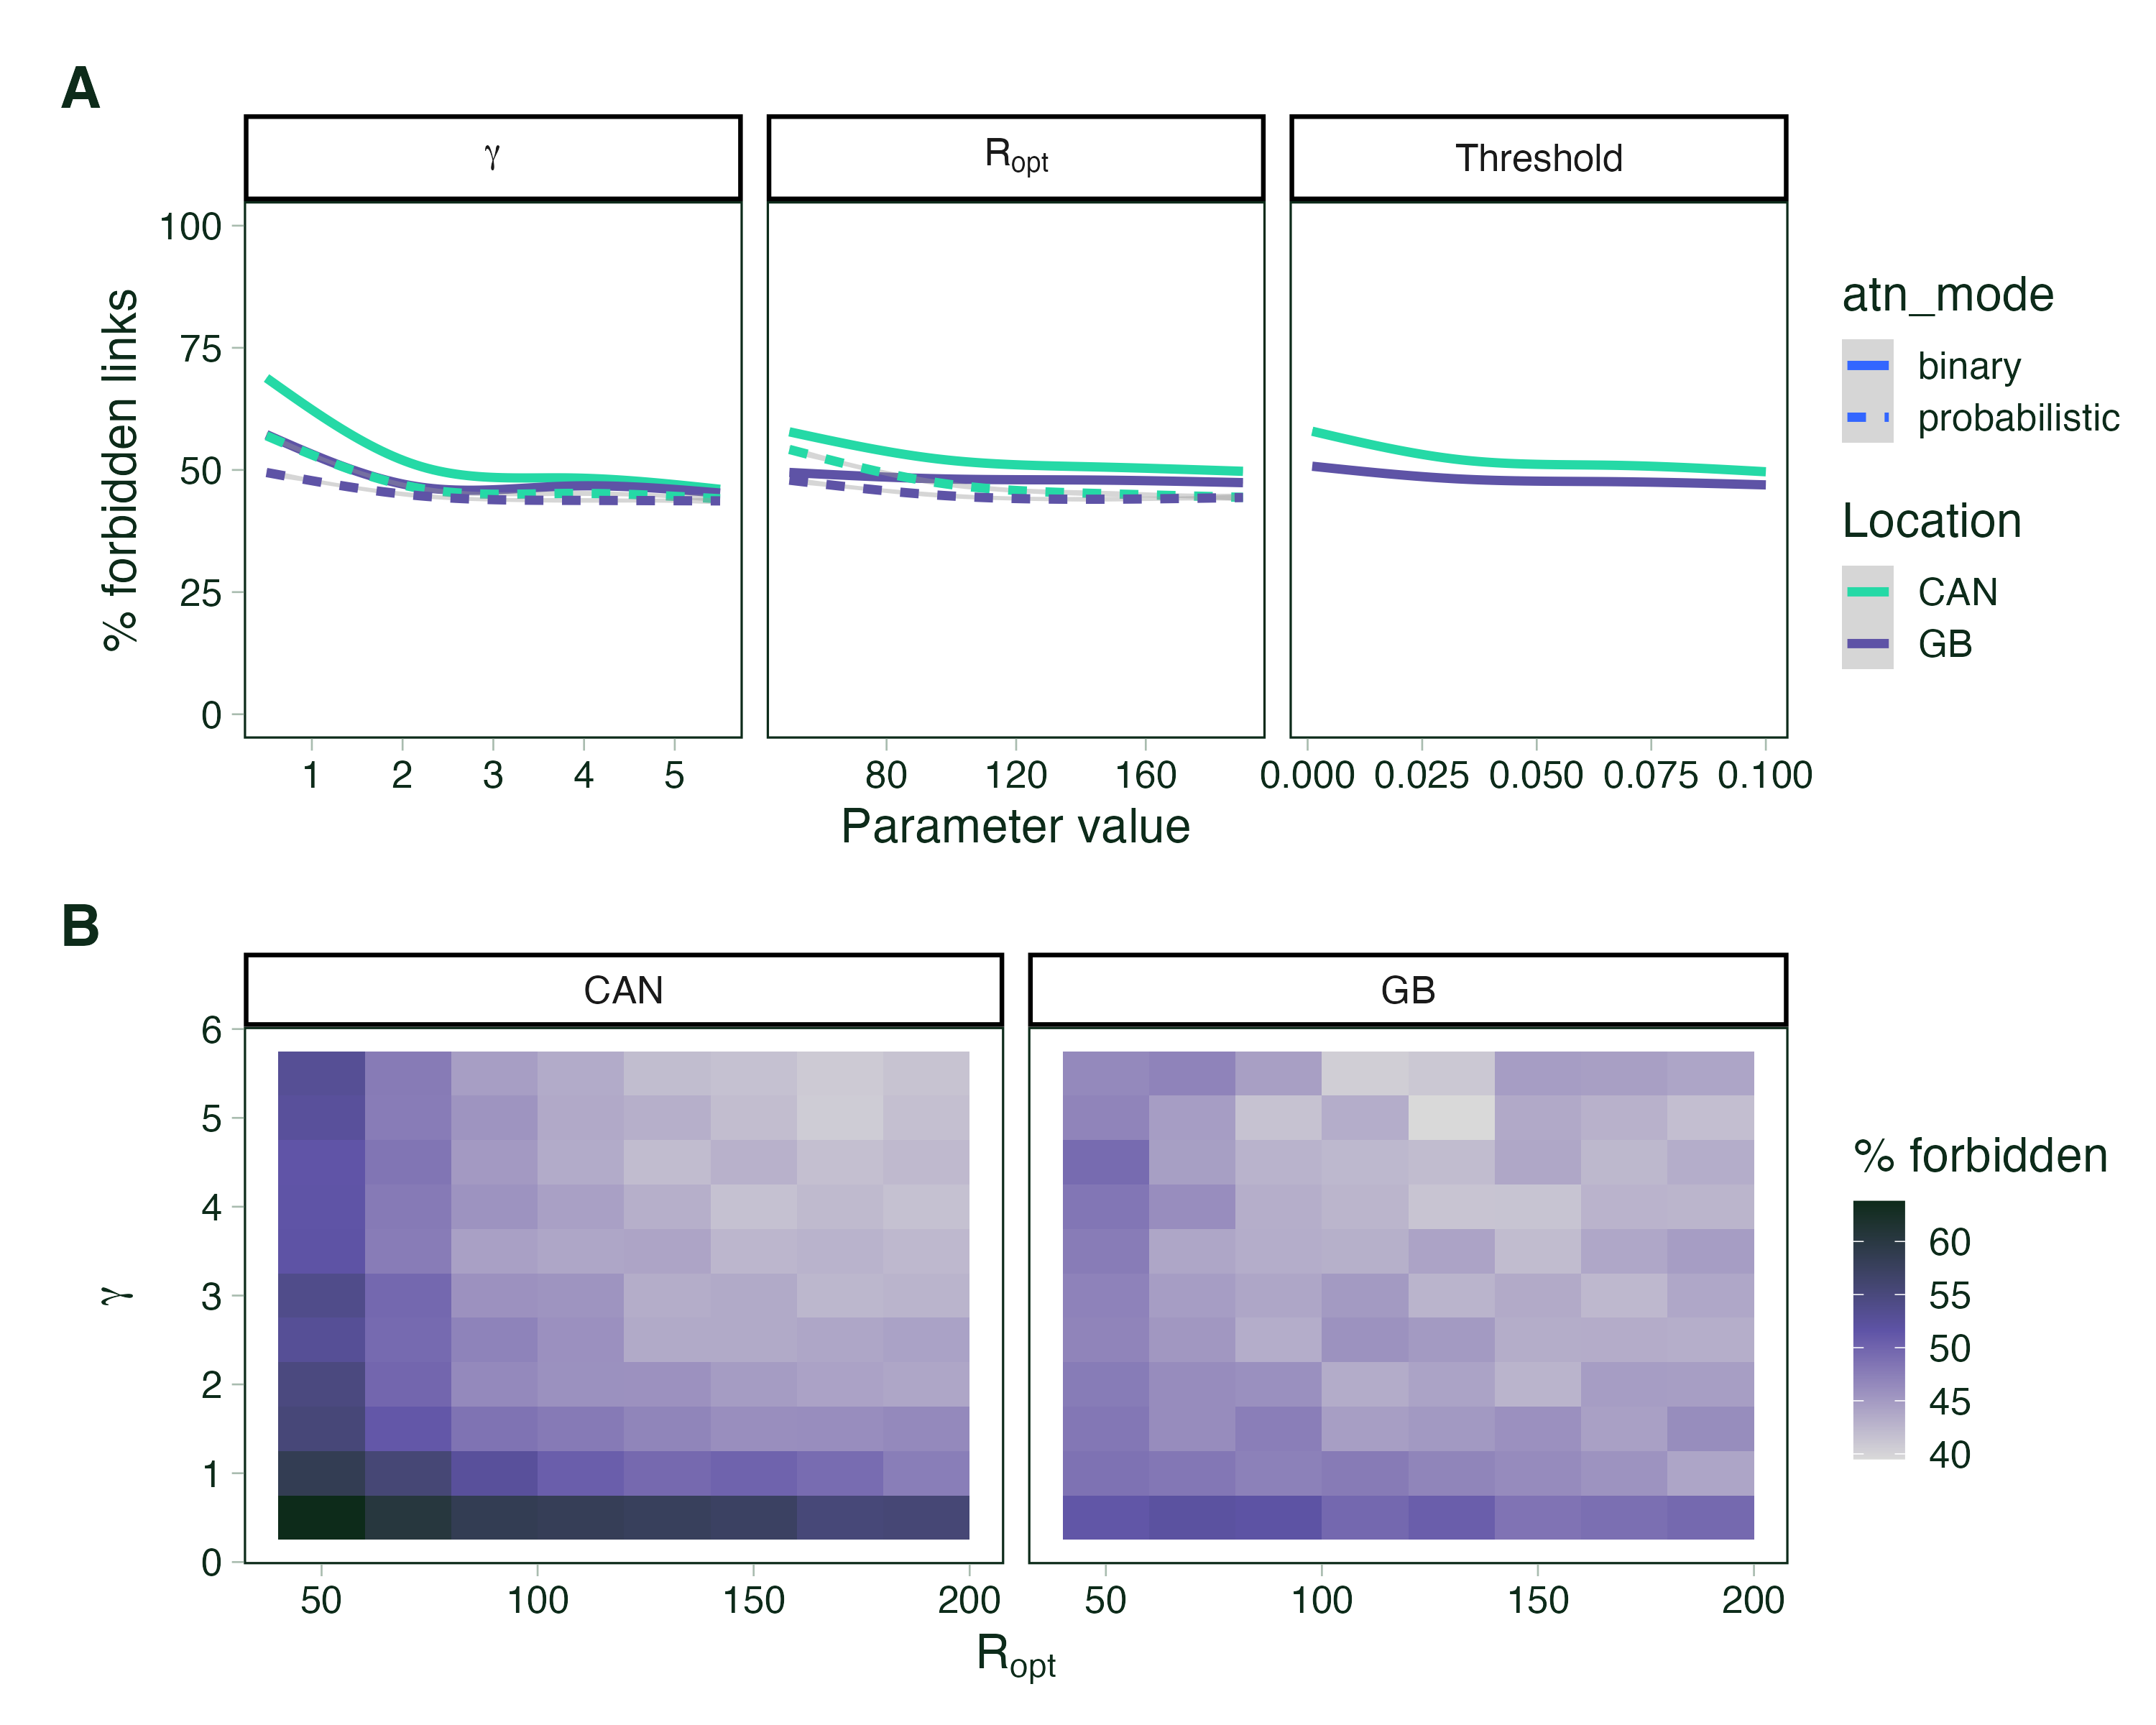
\includegraphics[keepaspectratio]{figures/forbidden_links.png}}

}

\caption{\label{fig-forbidden}\textbf{Sensitivity of ATN-predicted
forbidden interactions to model parameterisation}. (\textbf{A})
Percentage of predicted ATN interactions absent from the reference
metaweb (`forbidden links') across values of optimal predator--prey
body-mass ratio (\(R_{opt}\)), the body-mass scaling parameter
(\(\gamma\)), and the interaction-probability threshold. Lines show
trends across parameter values, with results distinguished by region and
ATN type; shaded bands indicate {[}95\% confidence intervals / standard
errors, as appropriate{]}. (\textbf{B}) Mean percentage of forbidden
links in probabilistic ATNs across combinations of \(R_{opt}\) and
\(\gamma\), with colour indicating the mean across simulation runs. For
Canada, ATN predictions were compared with the corresponding sampled
binary realisation of the probabilistic reference metaweb; for Great
Britain, predictions were compared with the fixed binary reference
metaweb. Forbidden-link percentage was calculated as the number of
predicted links absent from the reference metaweb divided by the total
number of predicted ATN links, multiplied by 100. Higher values indicate
that a greater proportion of predicted interactions are absent from the
reference metaweb.}

\end{figure}%

\section{Similar structure does not imply correct
interactions}\label{similar-structure-does-not-imply-correct-interactions}

\begin{itemize}
\tightlist
\item
  Compare structural metrics between ATN networks and metawebs.
\item
  Highlight any cases where structural similarity coexists with low
  pairwise interaction agreement.
\end{itemize}

\begin{figure}

\centering{

\pandocbounded{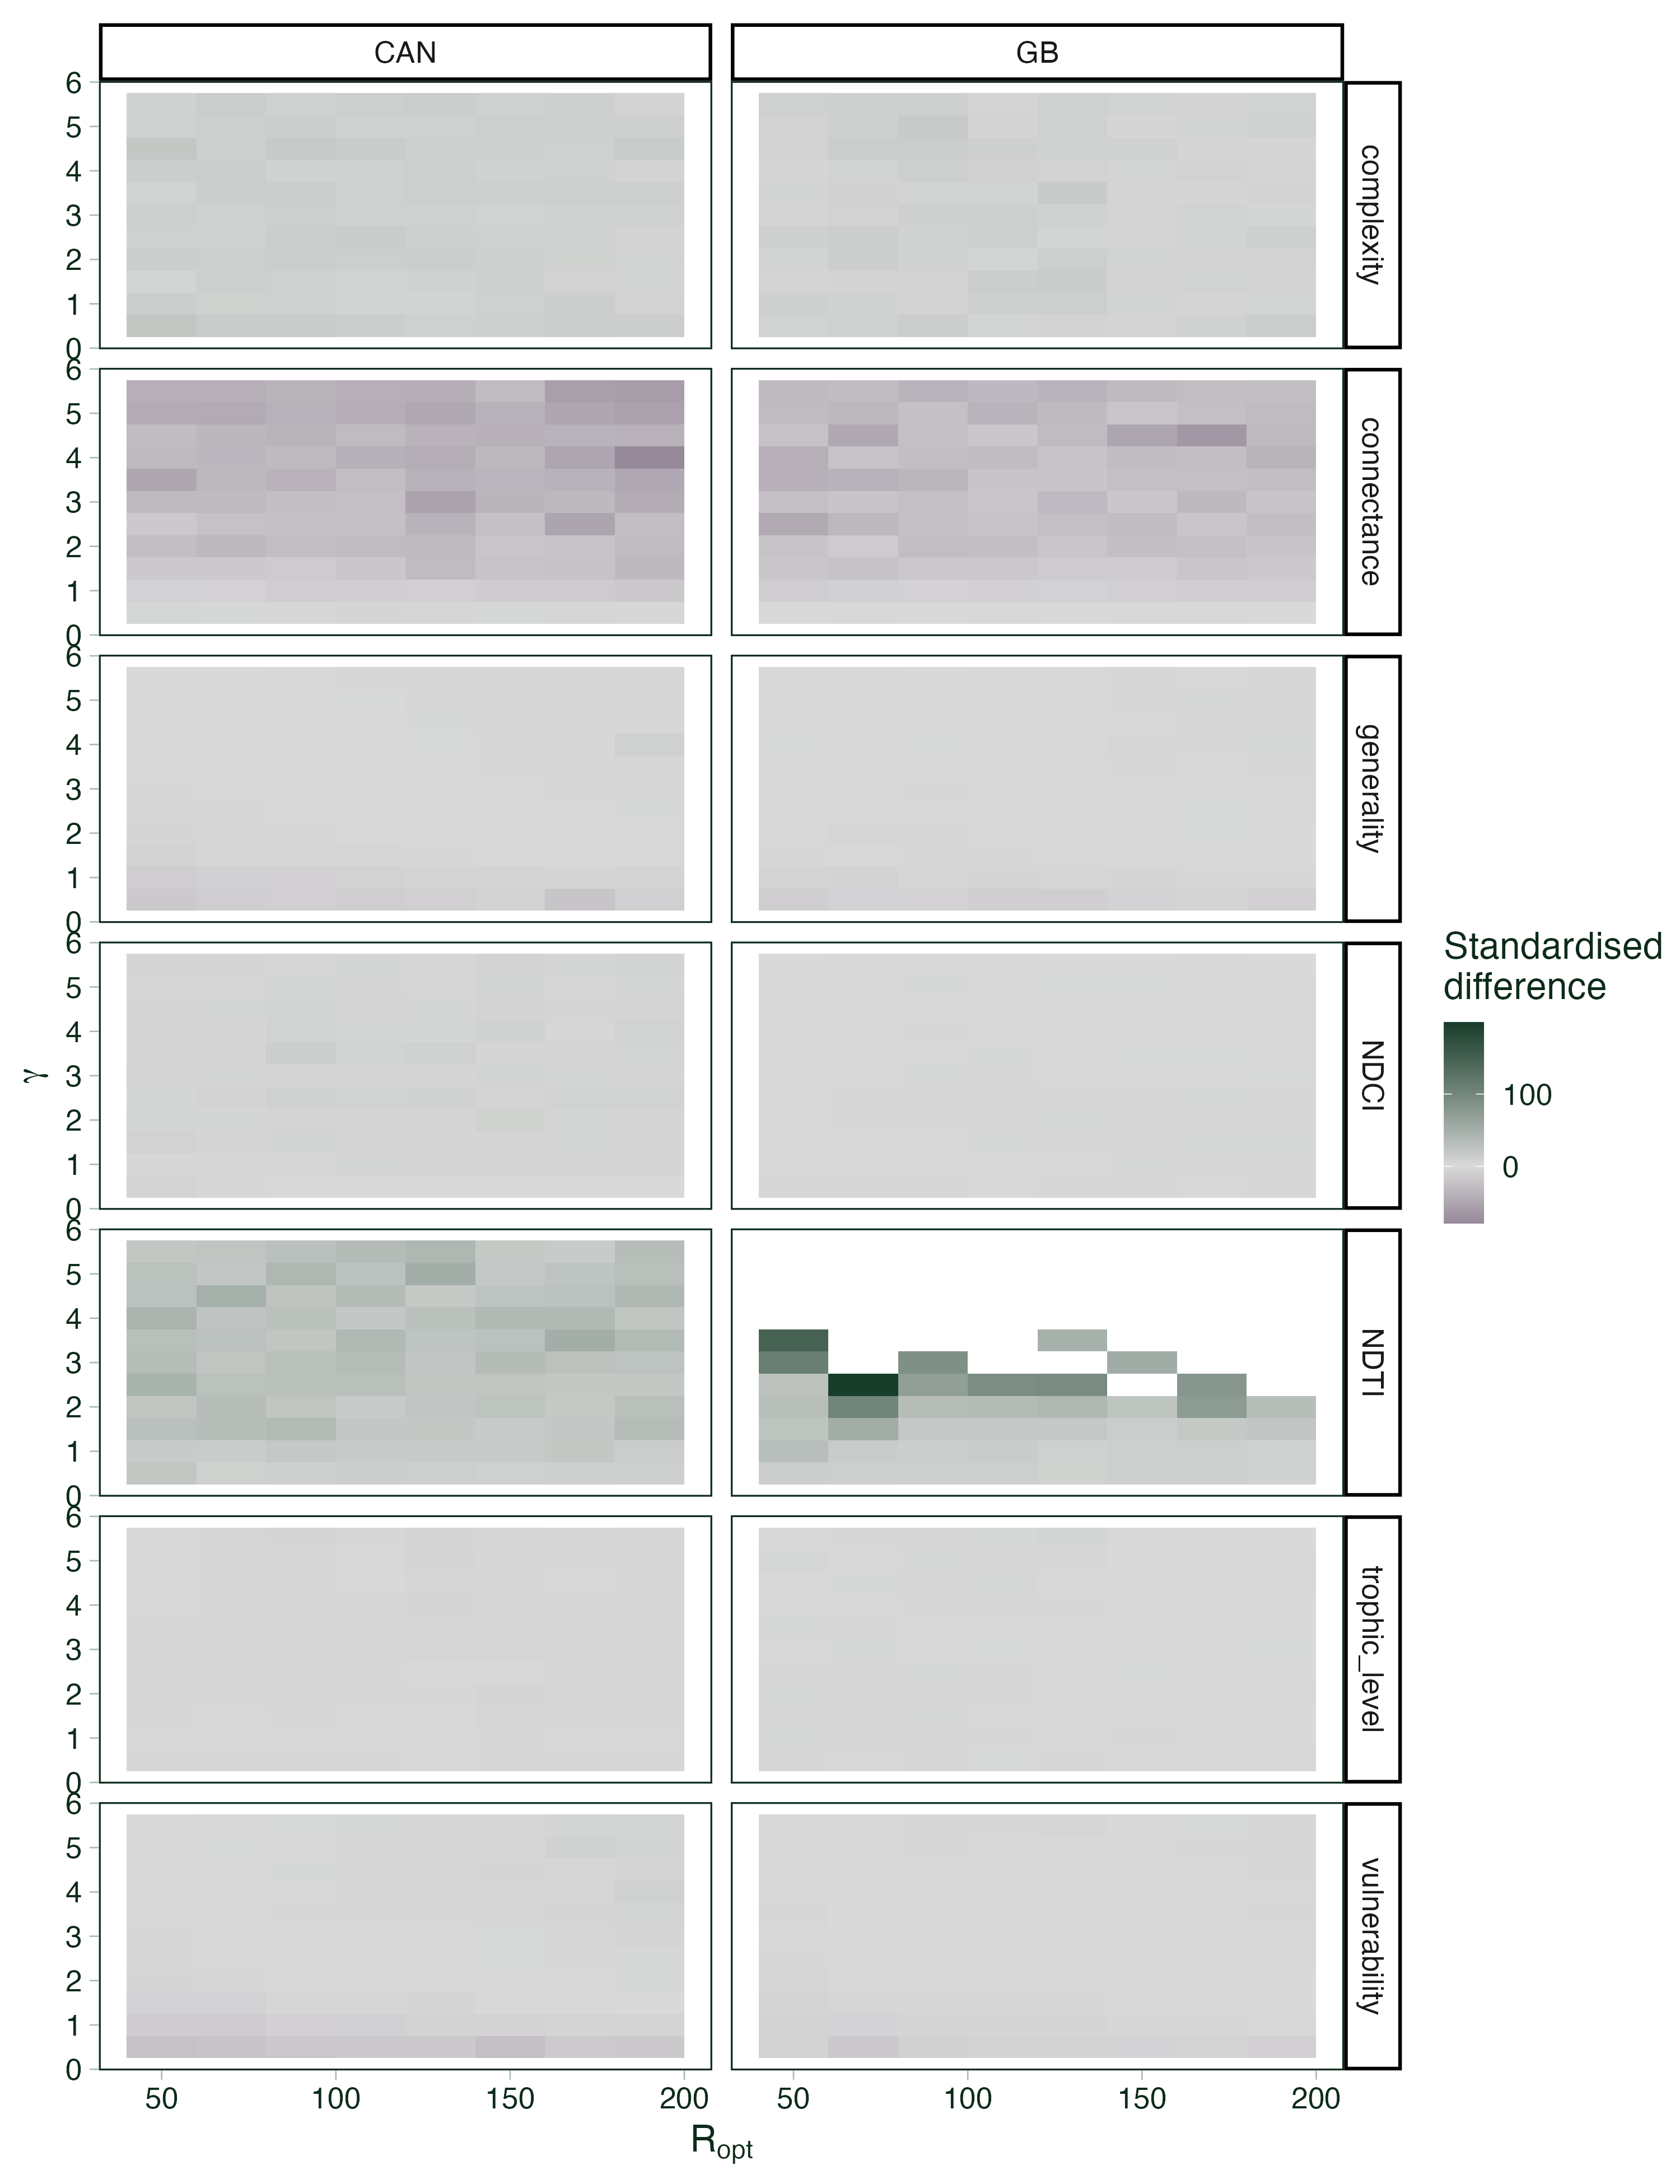
\includegraphics[keepaspectratio]{figures/strucutre.png}}

}

\caption{\label{fig-strucutre}Differences in network topology between
probabilistic ATN simulations and their corresponding metawebs across
values of optimal resource density (\(R_{opt}\)) and metabolic scaling
exponent (\(\gamma\)) for Great Britain (GB) and Canada (CAN). Tiles
show the mean standardised difference for seven network metrics:
connectance, complexity, trophic level, generality, vulnerability,
number of diet-trophic interactions (NDTI) and number of
diet-competition interactions (NDCI). Differences were calculated as ATN
minus metaweb values and standardised by the standard deviation of
differences across simulation runs for each parameter combination. For
GB, ATNs were compared with the fixed reference metaweb; for CAN, each
ATN was compared with its corresponding sampled metaweb. Values around
zero indicate smaller differences relative to the variability among
runs, while positive and negative values indicate higher and lower ATN
metric values, respectively, relative to the metaweb..}

\end{figure}%

\section{Discussion}\label{discussion}

\begin{itemize}
\tightlist
\item
  Body-size-based ATN models can predict interactions that are
  unsupported by the reference metawebs.
\item
  Structural similarity, if observed, does not necessarily imply
  recovery of the correct species-level links.
\item
  Discuss the limitations of body size as a sole predictor and the
  potential importance of additional traits and ecological constraints.
\item
  Note that metaweb absence is not definitive proof that an interaction
  is biologically impossible; results measure disagreement with the
  reference interaction data.
\end{itemize}

\section{Data and code availability}\label{data-and-code-availability}

\begin{itemize}
\tightlist
\item
  Provide data sources, analysis code and processed outputs.
\end{itemize}

\section*{References}\label{references}
\addcontentsline{toc}{section}{References}

\protect\phantomsection\label{refs}
\begin{CSLReferences}{1}{0}
\bibitem[\citeproctext]{ref-broseConsumerResourceBodySize2006}
Brose, U., Jonsson, T., Berlow, E. L., Warren, P., Banasek-Richter, C.,
Bersier, L.-F., Blanchard, J. L., Brey, T., Carpenter, S. R.,
Blandenier, M.-F. C., Cushing, L., Dawah, H. A., Dell, T., Edwards, F.,
Harper-Smith, S., Jacob, U., Ledger, M. E., Martinez, N. D., Memmott,
J., \ldots{} Cohen, J. E. (2006). Consumer--{Resource Body-Size
Relationships} in {Natural Food Webs}. \emph{Ecology}, \emph{87}(10),
2411--2417.
\url{https://doi.org/10.1890/0012-9658(2006)87\%5B2411:CBRINF\%5D2.0.CO;2}

\bibitem[\citeproctext]{ref-dansereauSpatiallyExplicitPredictions2024}
Dansereau, G., Barros, C., \& Poisot, T. (2024). Spatially explicit
predictions of food web structure from regional-level data.
\emph{Philosophical Transactions of the Royal Society B: Biological
Sciences}, \emph{379}(1909).
\url{https://doi.org/10.1098/rstb.2023.0166}

\bibitem[\citeproctext]{ref-jonesPanTHERIASpecieslevelDatabase2009}
Jones, K. E., Bielby, J., Cardillo, M., Fritz, S. A., O'Dell, J., Orme,
C. D. L., Safi, K., Sechrest, W., Boakes, E. H., Carbone, C., Connolly,
C., Cutts, M. J., Foster, J. K., Grenyer, R., Habib, M., Plaster, C. A.,
Price, S. A., Rigby, E. A., Rist, J., \ldots{} Purvis, A. (2009).
{PanTHERIA}: A species‐level database of life history, ecology, and
geography of extant and recently extinct mammals: {Ecological Archives
E090}‐184. \emph{Ecology}, \emph{90}(9), 2648--2648.
\url{https://doi.org/10.1890/08-1494.1}

\bibitem[\citeproctext]{ref-maioranoTETRAEU10Specieslevel2020a}
Maiorano, L., Montemaggiori, A., Ficetola, G. F., O'Connor, L., \&
Thuiller, W. (2020). {TETRA}‐{EU} 1.0: {A} species‐level trophic metaweb
of {European} tetrapods. \emph{Global Ecology and Biogeography},
\emph{29}(9), 1452--1457. \url{https://doi.org/10.1111/geb.13138}

\bibitem[\citeproctext]{ref-strydomFoodWebReconstruction2022}
Strydom, T., Bouskila, S., Banville, F., Barros, C., Caron, D., Farrell,
M. J., Fortin, M.-J., Hemming, V., Mercier, B., Pollock, L. J., Runghen,
R., Dalla Riva, G. V., \& Poisot, T. (2022). Food web reconstruction
through phylogenetic transfer of low-rank network representation.
\emph{Methods in Ecology and Evolution}, \emph{13}(12).
\url{https://doi.org/10.1111/2041-210X.13835}

\bibitem[\citeproctext]{ref-strydomSVDEntropyReveals2021}
Strydom, T., Dalla Riva, G. V., \& Poisot, T. (2021). {SVD Entropy
Reveals} the {High Complexity} of {Ecological Networks}. \emph{Frontiers
in Ecology and Evolution}, \emph{9}.
\url{https://doi.org/10.3389/fevo.2021.623141}

\end{CSLReferences}




\end{document}
